One of the main features of \mitobo and \alida, respectively, is their capability of automatically documenting data processing
pipelines. The operator concept allows to get a detailed internal log of all data manipulations, which
can subsequently be used to convert the
process history into a directed graph data structure denoted {\em history graph} in the following.
 
The \mitobo\ operator concept defines operators as the only places where data are processed and manipulated. 
Each call to an operator is associated with a certain configuration of the operator, defined by its {\em parameters}. 
The operator receives a number of objects as input parameters, 
which for example may be images or segmentation results like regions. The behaviour of the operator is controlled by control 
parameters, for example the size of a structuring element or a threshold. 
Finally, the operator produces output data, in particular images, but also for example numerical data,
regions or contours.

In \mitobo\ an image analysis pipeline usually consists of a set of different operators that are applied to incoming data and
produce result data. The order in which the operators work on the data depends on the specific pipeline. The invocation of
operators can be of pure sequential nature or subsume parallel processing steps. In addition, a nested application
of operators is possible. Given this principle each analysis pipeline and its
data flow may be interpreted
and visualized as a directed acyclic graph (cf.~Fig.~\ref{fig:DAG} for an
example).

A \mitobo\ history graph basically consists of operator and data nodes which are connected by edges 
indicating the flow of data, as can be seen from Fig.~\ref{fig:DAG}. 
The figure shows a screenshot of \mtbc which is a graph visualization tool derived from {\em Chisio}\footnote{
Chisio website, \href{http://sourceforge.net/projects/chisio}{http://sourceforge.net/projects/chisio}}.
Chisio is a graph visualization and editing tool written in Java which we extended for the specific needs of \alida and 
\mitobo history graphs.
More detailed information about \mtbc and its installation and usage can be found on the \alida webpage and in particular 
in \alida's user guide.

Within the history graph each operator node, which is linked to the {\em call} of a specific operator,
is depicted as a rectangle with the operator's 
classname in the bottom line,
For each input and output parameter object the operator node features input and output ports which may be conceived as the entry or exit points of data into and out of the operator. These ports are depicted as filled ellipses in light green (input ports) and dark green (output ports),
respectively. Each input port has exactly one incoming edge, while an output
port may be connected to multiple target ports,
depending on where the data is passed to. In Fig.~\ref{fig:DAG} the result
image 'resultImg' produced in the {\tt MTBMedian}
operator is handed over to the {\tt ActiveContours} operator as well as
returned directly to the calling operator
{\tt CellSegmentation}. Each port of an operator has an individual name indicating the input or output object associated
with the port. This allows to distinguish between ports if one operator defines multiple input ports as is
the case for the {\tt ActiveContours} operator.
\begin{center}
\begin{figure}
\vspace*{-0.85cm}
\centerline{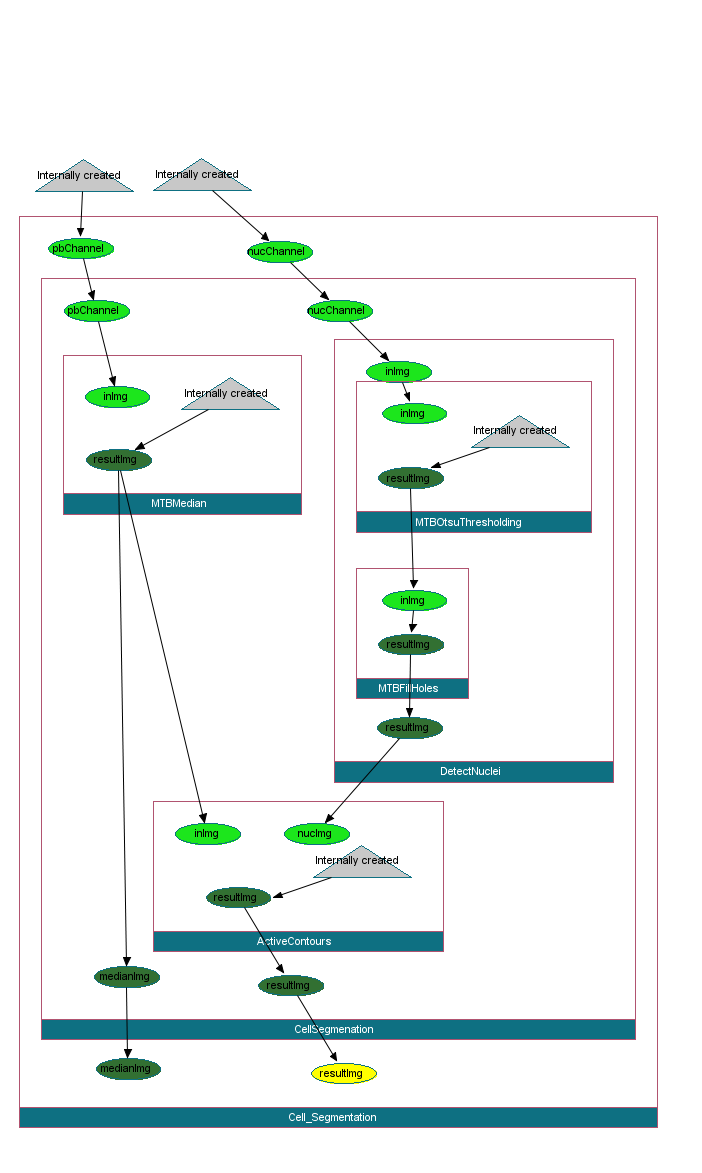
\includegraphics[clip, trim= 0 0 20 110, width=0.9\textwidth]{../images/exampleDAG.png}}
\vspace*{-0.85cm}
\caption[Example of a history graph.]{\label{fig:DAG}
A \mitobo\ history graph: the directed acyclic graph represents the application of nested operators. 
Calls to operators are depicted as rectangles, input and output ports as ellipses filled in light or dark green,
respectively. 
The grey triangles relate to newly generated data objects, and the yellow ellipse indicates the result data object
to which this history graph is linked to.}
\end{figure}
\end{center}

\vspace*{-1.25cm}
In addition to operator nodes and their ports there are also data nodes in the graph 
corresponding to the creation of new data objects, e.g., when data is read from
file, cloned or generated from scratch. These are depicted as triangles filled
in light grey.
In Fig.~\ref{fig:DAG} two data objects are created outside of the
processing pipeline as a result of reading images (at the top of the figure) and
are passed as input data objects to the {\tt Cell\_Segmentation} operator. 
Additionally, three more images are created by the operators {\tt MTBMedian}, {\tt MTBOtsuThresholding} and {\tt
ActiveContours} which in all three cases form the resulting data objects of these operators
and are passed to the outside via output ports.

Fig.~\ref{fig:DAG} shows the history graph for the output object 'resultImg' of
the operator {\tt Cell\_Segmentation}, where the corresponding port is shown as
a yellow ellipse at the bottom of the figure.
This history subsumes the calls of seven operators in total where some of these
calls are nested. The outmost operator is {\tt Cell\_Segmentation} which was
implemented as a \mitobo\ plugin, indicated by the underscore in its name
(cf.~Chap.~\ref{chap:ImplPlugins}). This plugin calls the {\tt CellSegmentation}
operator implementing the actual algorithms. For cell segmentation two input
images are required whereas one of these images is median
filtered by {\tt MTBMedian} while the second one is fed into the {\tt
DetectNuclei} operator. Inside of that operator
first {\tt MTBOtsuThresholding} is called, and the binary result image is subsequently post-processed applying {\tt
MTBFillHoles}. Its result is handed back to the calling {\tt DetectNuclei} operator and also directly propagated further back
to the {\tt CellSegmentation} operator. This operator finally calls the {\tt ActiveContours} operator which
generates one of the two result images of {\tt CellSegmentation}. The second result image is the median
filtered image which is also returned to the calling plugin as mentioned above.

The history data is stored in XML format in a file accompanying the actual data object file. 
The format basically relies on {\em GraphML}\footnote{GraphML website, 
\href{http://graphml.graphdrawing.org/}{http://graphml.graphdrawing.org/}} with some \alida and \mitobo\
specific extensions. When reading and writing images using \mitobo's {\tt 'Open\_Image\_MTB'} and {\tt 'Save\_Image\_MTB'} plugins,
or directly its {\tt 'ImageReaderMTB'} and {\tt 'ImageWriterMTB'} operators, respectively, history files are automatically considered. For example, for an image stored in the file '{\tt
example.tiff}' its history data is automatically saved to the accompanying file
'{\tt example.ald}'. The extension '{\tt
.ald}' indicates a {\em \mitobo\ processing history} file and in fact is derived from \alida, which is responsible for the 
processing histories in \mitobo. When later on reading the image using {\tt 'Open\_Image\_MTB'} or {\tt 'ImageReaderMTB'},
\mitobo's open operator checks for an accompanying file, and if one is found it is read and the corresponding history data is linked to the
image object. This allows to trace the processing history of an object in the
long run and even when the
processing pipeline was interrupted by intermediate savings of data to disk.

Note, the identity of images is {\em not} preserved in the processing history
across file boundaries. If two (or more) input images for the current top
level operator (in Fig.~\ref{fig:DAG} this would be the operator {\tt Cell\_Segmentation}), are loaded
from the same image file, both will nevertheless be displayed as different data
nodes in the history. The reason is that object identity is not -- and maybe even cannot -- be checked from the
processing history of former operations.

\paragraph{Important Note:}
At the moment, with regard to ImageJ, automatic process documentation is only supported for operators and plugins from
\mitobo\ itself, i.e.~intermediate calls to pure ImageJ functions are not documented and may corrupt the processing history. 
Contrary, in ImageJ $2.0$ also calls to ImageJ $2.0$ plugins are included in the history. But note that in both cases,
to make use of the automatic documentation to its full extent, it is indispensable to use the I/O operators of \mitobo\ to open 
input data and save the resulting output data as the ImageJ and ImageJ $2.0$ I/O functions do not know anything about histories. 
